\section*{Conclusions}

The first important conclusion that come to mind is the fact that a problem that has no solution can be verified. Complexity theory has taught us that there can be a large gap between the complexity of verification versus search, but it has always been a difference of efficiency: if solutions to a problem can be verified then solutions can also be found (even if with drastically higher computational cost). This result show us that, with quantum entanglement, there can be a chasm of computability between verifying solutions and finding them.


There are still many things that are not clear. First of all: what is the role of entanglement here. What we have shown goes in the opposite direction of what the result seems to be. Entanglement makes the provers even more powerful, but in the end seems to make the verifier more efficient.

We also quickly mention some open questions:
\begin{itemize}

    \item To this day, nobody built an explicit $II_1$ factor that doesn't satisfy Connes'embedding property.
    \item We could consider the complexity class $\text{MIP}^\text{co}$, which stands for \emph{multiprover interactive proofs in the commuting-operator model}. As always, we consider only two-prover one-round protocols. We know that this is contained in co-RE, namely the complement of RE. One could ask if $\text{MIP}^\text{co}$ = co-RE sussist.
    
\end{itemize}

Finally an important conclusion is that it seems like quantum computer are inherently more powerful in verifying problem rather than solving problem. Let us explain.

At the moment we have the following situation: there are some evidence~\cite{Bennett_1997} that $\textbf{BQP} \neq \textbf{BPP}$ (i.e. polynomial-time quantum Turing machines are more powerful than polynomial-time probabilistic Turing machines). Since \textbf{BPP} is regarded as the class of all efficiently computable languages, this provides evidence that quantum computers could be inherently more powerful than classical computers in a model-independent way.

However exactly where \textbf{BQP} fits with respect to \textbf{P}, \textbf{NP} and \textbf{PSPACE} is as yet unknown. What is known is that quantum computers can solve all the problems in \textbf{P} efficiently and that there are no problems outside of \textbf{PSPACE} which they can solve efficiently. Therefore, \textbf{BQP} lies somewhere between \textbf{P} and \textbf{PSPACE}.
It has been demonstrated that
\begin{equation*}
   \textbf{P}   \subseteq \textbf{BPP} \subseteq \textbf{BQP}  \subseteq \textbf{PSPACE}
\end{equation*}
note that this is not even close to be a speed improvement  as it is MIP*=RE, where, w.r.t. MIP, the power of verification is astonishingly enhanced.


\begin{figure}[htb]
    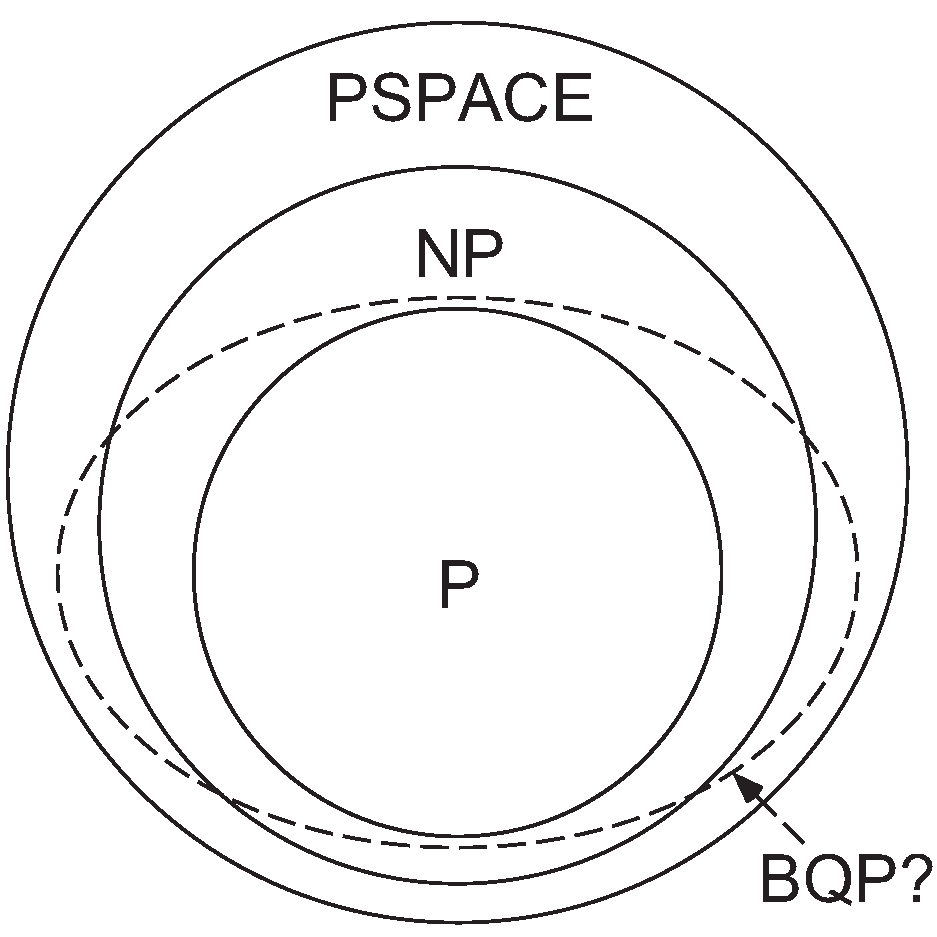
\includegraphics[width=\linewidth]{Quantum-complexity.png}
    \centering
    \caption{Complexity classes hierarchy.}
    \end{figure}